\documentclass[12pt,a4paper]{article}

\usepackage[a4paper,margin=1in]{geometry}
\usepackage{graphicx}
\usepackage{booktabs}
\usepackage{amsmath,amssymb}
\usepackage{float}
\usepackage{hyperref}
\usepackage{xcolor}
\usepackage{listings}
\usepackage{enumitem}
\usepackage{fancyhdr}
\usepackage{longtable}

\hypersetup{colorlinks=true,linkcolor=blue,urlcolor=blue}

\pagestyle{fancy}
\fancyhf{}
\lhead{ICS1512}
\rhead{Machine Learning Algorithms Laboratory}
\cfoot{\thepage}

% ===== Python syntax highlighting colors =====
\definecolor{codegreen}{rgb}{0,0.6,0}
\definecolor{codegray}{rgb}{0.5,0.5,0.5}
\definecolor{codepurple}{rgb}{0.58,0,0.82}
\definecolor{codeblue}{rgb}{0,0,0.8}
\definecolor{backcolour}{rgb}{0.95,0.95,0.92}

\lstset{
language=Python,
basicstyle=\ttfamily\small,
backgroundcolor=\color{backcolour},
commentstyle=\color{codegreen},
keywordstyle=\color{codeblue},
stringstyle=\color{codepurple},
numberstyle=\tiny\color{codegray},
numbers=left,
frame=single,
breaklines=true,
showstringspaces=false,
tabsize=4,
captionpos=b
}

\begin{document}

\begin{tabular}{|p{4cm}|p{11cm}|}
\hline
Experiment No. & 1 \\ \hline
Experiment Title &
Exploratory Data Analysis on Multiple Datasets
\footnote{\textbf{GitHub Repository: }\url{https://github.com/JJBOY12345/MLAssign_SSN/tree/main}}\\ \hline
Student Name  & J JESWIN JOEL \\ \hline
Register Number & 3122247001018  \\ \hline
Faculty & Dr. Poreddy Ajay Kumar Reddy \\ \hline
Submission Date & \\ \hline
\end{tabular}

\section{Objective}
Learn TO create modular function which can load and perform eda operation like histogram,pairplot,heatmap on the dataset.
\section{Tools and Libraries Used}
\begin{itemize}
    \item \textbf{Python Version}: Python 3.12.3
    \item \textbf{pandas}: For data loading, manipulation, and analysis
    \item \textbf{NumPy}: For numerical computations
    \item \textbf{Matplotlib}: For static visualizations
    \item \textbf{Seaborn}: For statistical visualizations
    \item \textbf{scikit-learn}: For loading built-in datasets (Digits)
    \item \textbf{IDE}: Vs code
\end{itemize}

\section{Generic Functions Implemented}
The following reusable functions were implemented to perform EDA across all datasets:

\begin{itemize}
    \item \texttt{load\_dataset()}: Loads a CSV file with optional column names and separator.
    \item \texttt{dataset\_info()}: Displays shape, column names, data types, memory usage, and first 5 rows.
    \item \texttt{missing\_values()}: Reports count and percentage of missing values per column.
    \item \texttt{duplicate\_info()}: Reports the number of duplicate rows.
    \item \texttt{summary\_statistics()}: Prints descriptive statistics for numerical columns.
    \item \texttt{class\_distribution()}: Plots a bar chart for a categorical/target column.
    \item \texttt{plot\_histogram()}: Plots histograms for all numerical features.
    \item \texttt{plot\_boxplot()}: Plots box plots for all numerical features to detect outliers.
    \item \texttt{plot\_heatmap()}: Plots a correlation heatmap for numerical features.
    \item \texttt{plot\_scatterplot()}: Plots a pair plot (scatter matrix) with optional hue.
    \item \texttt{perform\_eda()}: Orchestrates the full EDA pipeline with configurable options.
\end{itemize}

\subsection{Dataset Loading}

The \texttt{load\_dataset()} function is responsible for reading the dataset
from a CSV file while supporting optional column names and custom separators.

\begin{lstlisting}[language=Python,caption={Dataset Loading Function}]
def load_dataset(filepath, column_names=None, seperator=","):
    df = pd.read_csv(filepath,
                     names=column_names,
                     sep=seperator)
    df.columns = df.columns.str.strip()
    return df
\end{lstlisting}


\subsection{Dataset Information}

The \texttt{dataset\_info()} function displays the basic properties of the
dataset such as dimensions, column names, data types, memory usage and the
first few records.

\begin{lstlisting}[language=Python,caption={Dataset Information Function}]
def dataset_info(df):
    print(df.shape)
    print(df.columns.tolist())
    print(df.dtypes)
    df.info()
    print(df.head())
\end{lstlisting}


\subsection{Missing Value Analysis}

The following function computes the number and percentage of missing values
present in every feature.

\begin{lstlisting}[language=Python,caption={Missing Value Analysis}]
def missing_values(df):
    missing = df.isnull().sum()
    percent = (missing/len(df))*100

    result = pd.DataFrame({
        "missing": missing,
        "percent": percent
    })

    return result
\end{lstlisting}


\subsection{Duplicate Record Detection}

This function determines the number of duplicate records present in the dataset.

\begin{lstlisting}[language=Python,caption={Duplicate Detection}]
def duplicate_info(df):
    duplicates = df.duplicated().sum()
    return duplicates
\end{lstlisting}


\subsection{Summary Statistics}

The following function generates descriptive statistics for all numerical
attributes.

\begin{lstlisting}[language=Python,caption={Summary Statistics}]
def summary_statistics(df):
    print(df.describe())
\end{lstlisting}


\subsection{Class Distribution}

The class distribution function visualizes the frequency of each class in the
target variable.

\begin{lstlisting}[language=Python,caption={Class Distribution}]
def class_distribution(df, target_column):
    counts = df[target_column].value_counts()
    counts.plot(kind="bar")
    plt.show()
\end{lstlisting}


\subsection{Histogram Visualization}

Histograms are generated for every numerical feature to study their
distributions.

\begin{lstlisting}[language=Python,caption={Histogram Plot}]
def plot_histogram(df, bins=10):
    numeric_df = df.select_dtypes("number")
    numeric_df.hist(bins=bins)
    plt.show()
\end{lstlisting}


\subsection{Box Plot Visualization}

Box plots are used to identify the spread of data and detect possible outliers.

\begin{lstlisting}[language=Python,caption={Box Plot}]
def plot_boxplot(df):
    numeric_df = df.select_dtypes("number")

    for col in numeric_df.columns:
        plt.boxplot(numeric_df[col])
        plt.show()
\end{lstlisting}


\subsection{Correlation Heatmap}

The heatmap visualizes the correlation among numerical features.

\begin{lstlisting}[language=Python,caption={Correlation Heatmap}]
def plot_heatmap(df):
    numeric_df = df.select_dtypes("number")
    corr = numeric_df.corr()
    sns.heatmap(corr, annot=True)
    plt.show()
\end{lstlisting}


\subsection{Pair Plot Visualization}

Pair plots help visualize pairwise relationships among features.

\begin{lstlisting}[language=Python,caption={Pair Plot}]
def plot_scatterplot(df, target_column=None):

    if target_column is not None:
        sns.pairplot(df, hue=target_column)
    else:
        sns.pairplot(df)

    plt.show()
\end{lstlisting}


\subsection{Integrated EDA Pipeline}

The \texttt{perform\_eda()} function integrates all reusable EDA functions into
a single configurable workflow.

\begin{lstlisting}[language=Python,caption={Integrated EDA Pipeline}]
def perform_eda(...):

    df = load_dataset(...)

    dataset_info(df)
    missing_values(df)
    duplicate_info(df)
    summary_statistics(df)

    ...

    plot_histogram(df)
    plot_boxplot(df)
    plot_heatmap(df)
    plot_scatterplot(df)

    return df
\end{lstlisting}

\section{Dataset 1: Iris Dataset (Classification)}

\subsection{Dataset Description}
\begin{longtable}{|p{5cm}|p{9cm}|}
\hline
Dataset Name & Iris \\ \hline
Dataset Source & \texttt{iris/iris.data} (UCI Repository) \\ \hline
Number of Samples & 150 \\ \hline
Number of Features & 4 (sepal\_length, sepal\_width, petal\_length, petal\_width) \\ \hline
Target Classes & 3 (Iris-setosa, Iris-versicolor, Iris-virginica) \\ \hline
Missing Values & None \\ \hline
Duplicate Records & 3 \\ \hline
\end{longtable}

% TODO: Describe the dataset, its features, and the classification task.

\subsection{Loading and Basic Information}
The dataset is loaded using the \texttt{load\_dataset()} function. This function accepts the dataset file path as input and reads the CSV file using \texttt{pd.read\_csv()}. After loading the data into a Pandas DataFrame, the column names are cleaned by removing any leading or trailing whitespace. Finally, the processed DataFrame is returned for further analysis.

\subsection{Missing Values and Duplicates}
In Iris dataset there is: 
\begin{itemize}
    \item No missing value
    \item 3 Duplicate values!
\end{itemize}

\subsection{Exploratory Data Analysis}

\subsubsection{Summary Statistics}
\begin{itemize}
    \item The sepal length has highest mean
    \item The petal length has highest standard deviation
    \item The petal width has minimum width of 0.1 which is really small!
\end{itemize}

\begin{longtable}{|l|r|r|r|r|}
\hline
\textbf{Feature} & \textbf{Mean} & \textbf{Std} & \textbf{Min} & \textbf{Max} \\ \hline
sepal\_length & 5.843 & 0.828 & 4.3 & 7.9 \\ \hline
sepal\_width  & 3.054 & 0.434 & 2.0 & 4.4 \\ \hline
petal\_length & 3.759 & 1.764 & 1.0 & 6.9 \\ \hline
petal\_width  & 1.199 & 0.763 & 0.1 & 2.5 \\ \hline
\end{longtable}

\subsubsection{Class Distribution}
\begin{figure}[H]
\centering
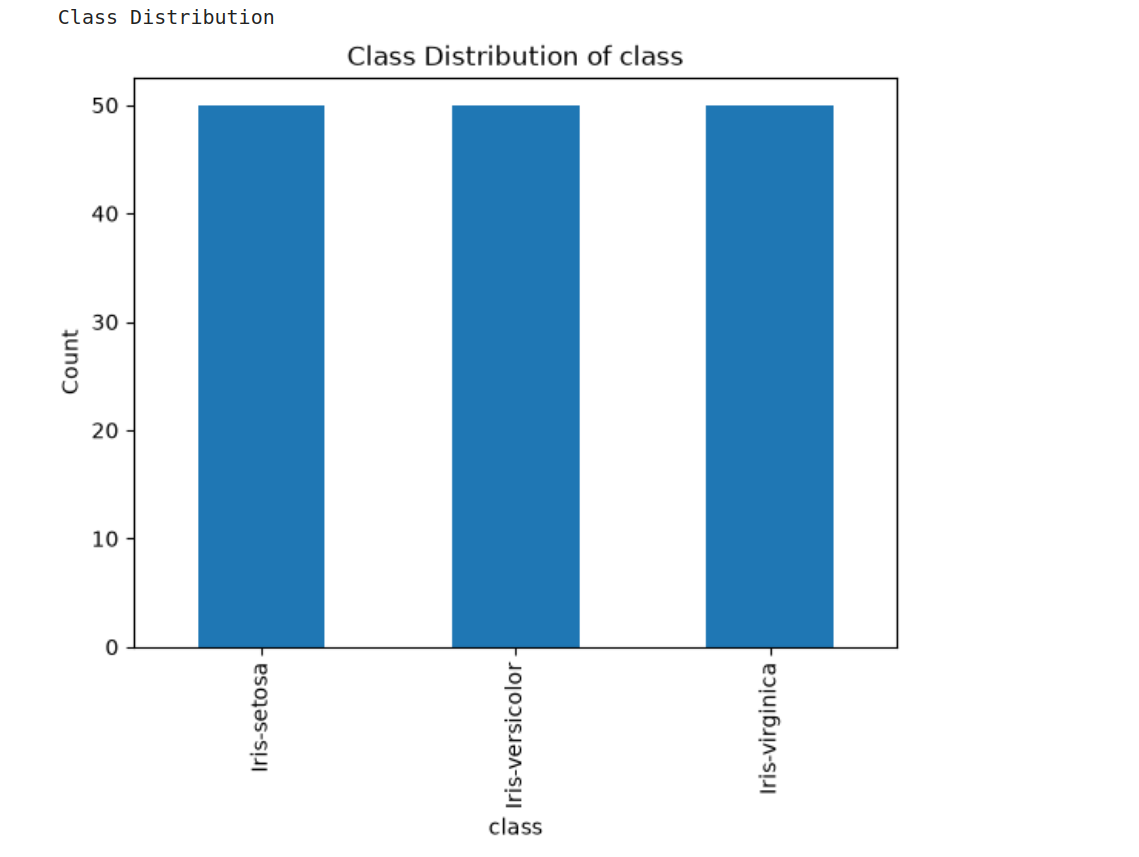
\includegraphics[width=0.7\linewidth]{images/iris_class_distribution.png}
\caption{Class Distribution of Iris Species}
\end{figure}

\textbf{Inference:}
TODO: Explain that each class has 50 samples, making the dataset balanced.

\subsubsection{Histograms}
\begin{figure}[H]
\centering
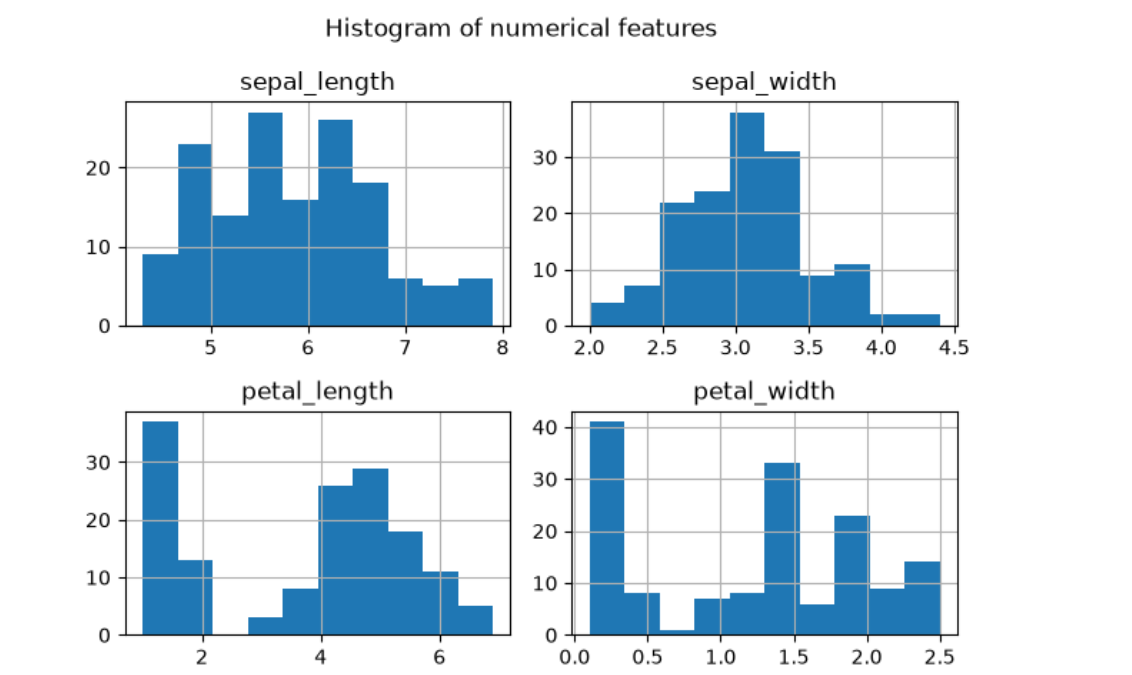
\includegraphics[width=0.7\linewidth]{images/iris_histograms.png}
\caption{Histograms of Numerical Features — Iris Dataset}
\end{figure}

\textbf{Inference:}
TODO: Describe the distribution shapes — petal length and petal width are bimodal, while sepal features are unimodal.

\subsubsection{Box Plots}
The \texttt{plot\_boxplot()} function generates one separate box plot per numerical feature. For Iris, 4 individual box plots were generated:

\begin{figure}[H]
\centering
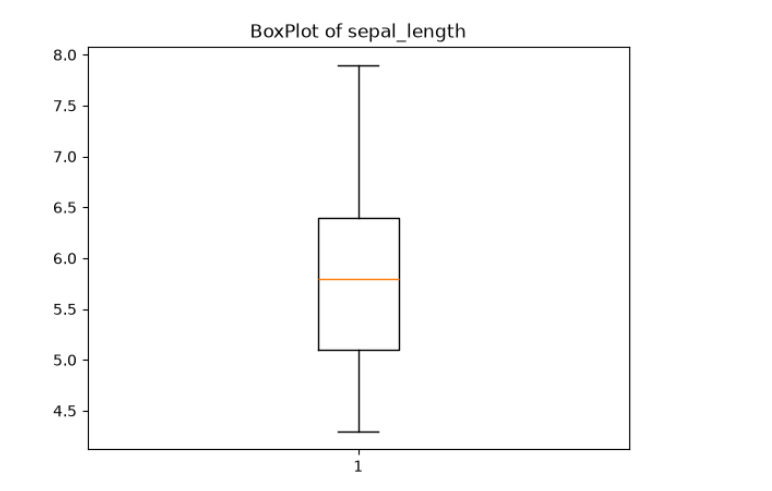
\includegraphics[width=0.6\linewidth]{images/iris_boxplot_sepal_length.png}
\caption{Box Plot of Sepal Length}
\end{figure}
\begin{figure}[H]
\centering
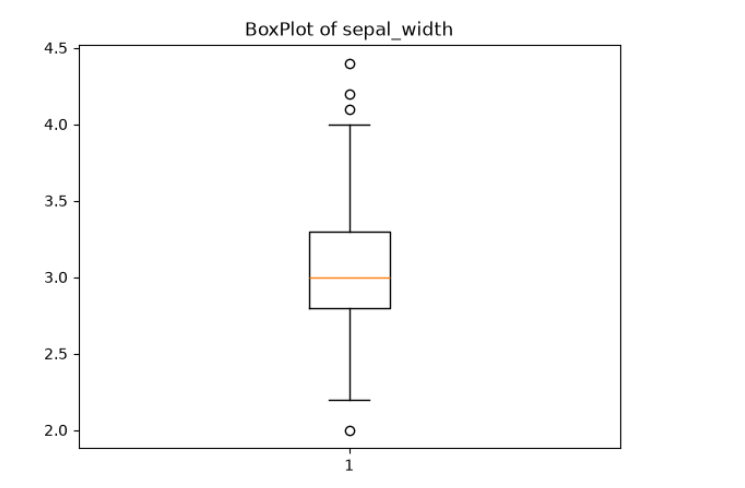
\includegraphics[width=0.6\linewidth]{images/iris_boxplot_sepal_width.png}
\caption{Box Plot of Sepal Width}
\end{figure}
\begin{figure}[H]
\centering
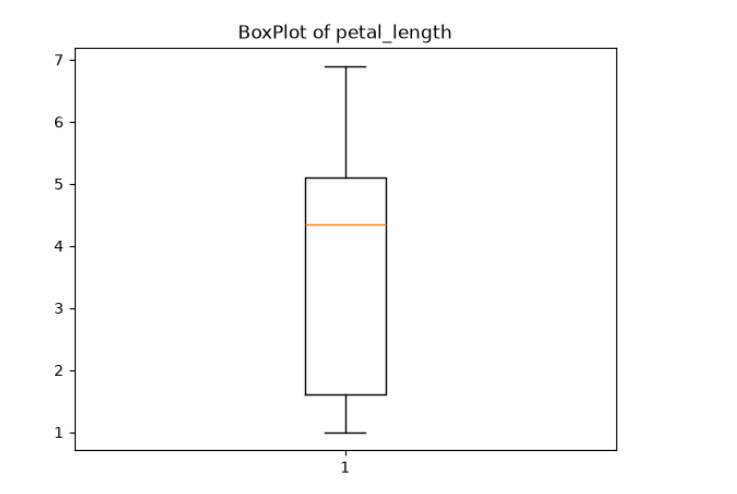
\includegraphics[width=0.6\linewidth]{images/iris_boxplot_petal_length.png}
\caption{Box Plot of Petal Length}
\end{figure}
\begin{figure}[H]
\centering
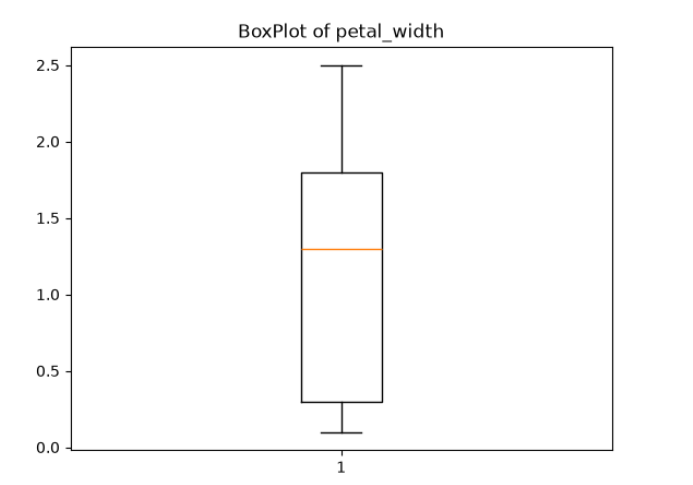
\includegraphics[width=0.6\linewidth]{images/iris_boxplot_petal_width.png}
\caption{Box Plot of Petal Width}
\end{figure}

\textbf{Inference:}
TODO: Discuss outliers observed — sepal width has outliers above 4.0 and below 2.0; the other three features show no outliers.

\subsubsection{Correlation Heatmap}
\begin{figure}[H]
\centering
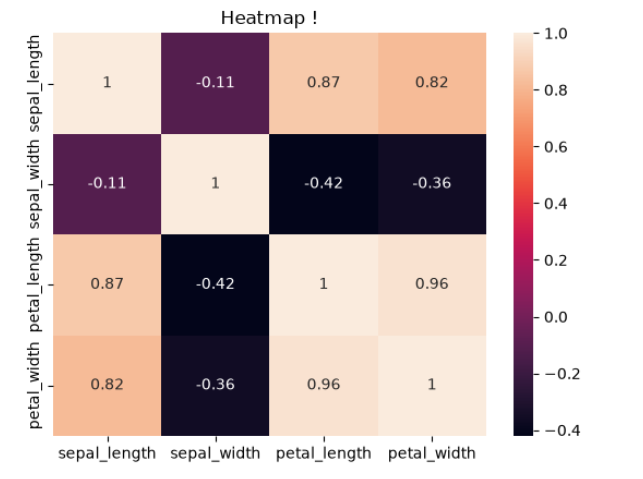
\includegraphics[width=0.7\linewidth]{images/iris_correlation_heatmap.png}
\caption{Correlation Heatmap — Iris Dataset}
\end{figure}

\textbf{Inference:}
TODO: Interpret the strong positive correlation between petal length and petal width (~0.96), and the weaker correlation with sepal width.

\subsubsection{Pair Plot}
\begin{figure}[H]
\centering
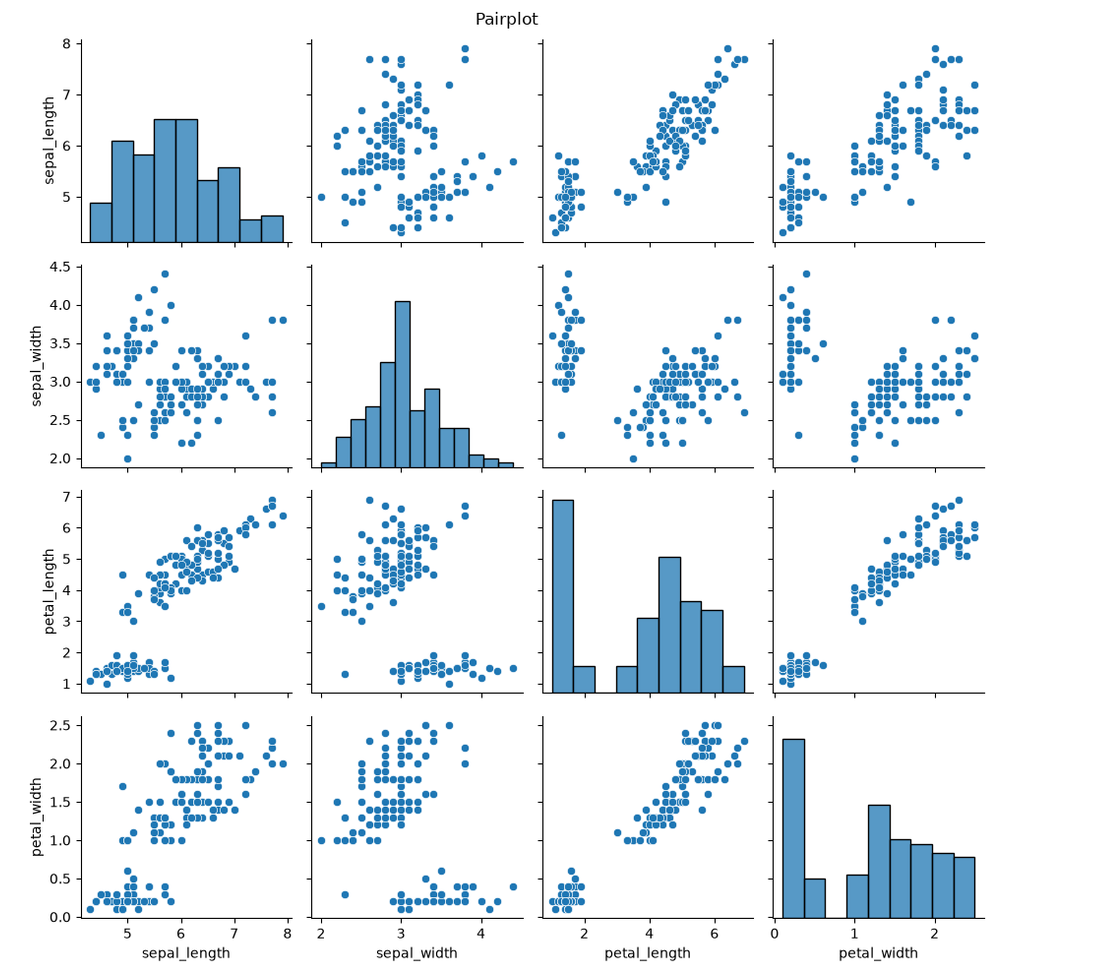
\includegraphics[width=0.7\linewidth]{images/iris_pairplot.png}
\caption{Pair Plot of All Features — Iris Dataset}
\end{figure}

\textbf{Inference:}
TODO: Describe how the pair plot reveals natural clustering among the species, especially in petal-related features.

\section{Dataset 2: Loan Approval Dataset (Classification)}

\subsection{Dataset Description}
\begin{longtable}{|p{5cm}|p{9cm}|}
\hline
Dataset Name & Loan Approval \\ \hline
Dataset Source & \texttt{LoanAmount/loan\_approval\_dataset.csv} \\ \hline
Number of Samples & 4,269 \\ \hline
Number of Features & 13 (10 numerical, 3 categorical) \\ \hline
Target Variable & \texttt{loan\_status} (Approved / Rejected) \\ \hline
Missing Values & None \\ \hline
Duplicate Records & None \\ \hline
\end{longtable}

TODO: Describe the dataset, the features, and the prediction task (loan approval classification).

\subsection{Loading and Basic Information}
TODO: Discuss the structure of the dataset, data types, and initial observations.

\subsection{Missing Values and Duplicates}
TODO: Report that no missing values or duplicates were found.

\subsection{Summary Statistics}
TODO: Present and interpret key statistics — income range, loan amount range, CIBIL scores, and the unusual negative value in residential assets.

\begin{longtable}{|l|r|r|r|r|}
\hline
\textbf{Feature} & \textbf{Mean} & \textbf{Std} & \textbf{Min} & \textbf{Max} \\ \hline
income\_annum & TODO & TODO & TODO & TODO \\ \hline
loan\_amount & TODO & TODO & TODO & TODO \\ \hline
cibil\_score & TODO & TODO & TODO & TODO \\ \hline
loan\_term & TODO & TODO & TODO & TODO \\ \hline
residential\_assets\_value & TODO & TODO & TODO & TODO \\ \hline
\end{longtable}

\subsection{Exploratory Data Analysis}

\subsubsection{Class Distribution — Loan Status}
\begin{figure}[H]
\centering
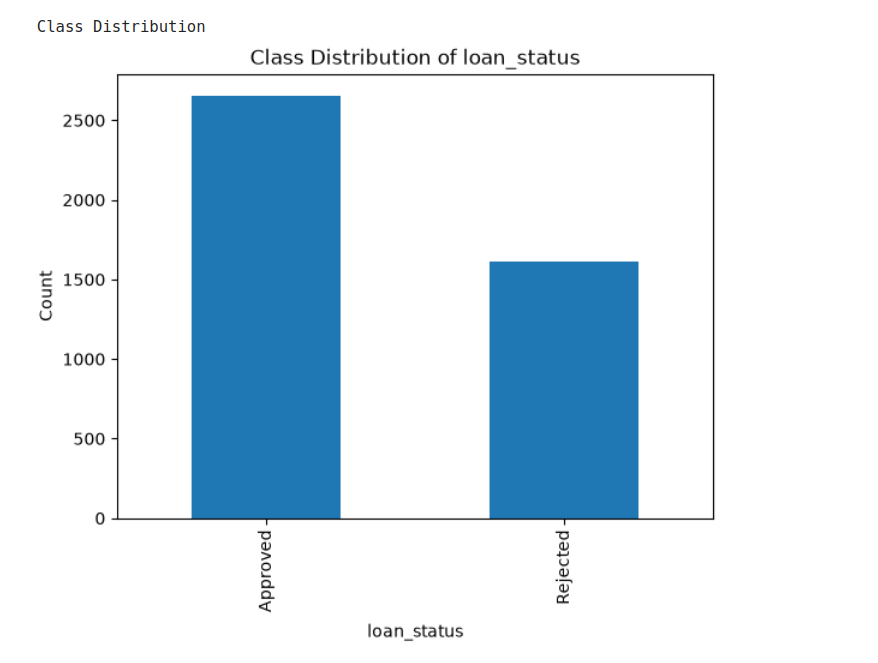
\includegraphics[width=0.7\linewidth]{images/loan_loan_status_distribution.png}
\caption{Distribution of Loan Status}
\end{figure}

\textbf{Inference:}
TODO: Discuss whether the dataset is balanced or imbalanced with respect to loan status.

\subsubsection{Class Distribution — Education and Self Employed}
\begin{figure}[H]
\centering
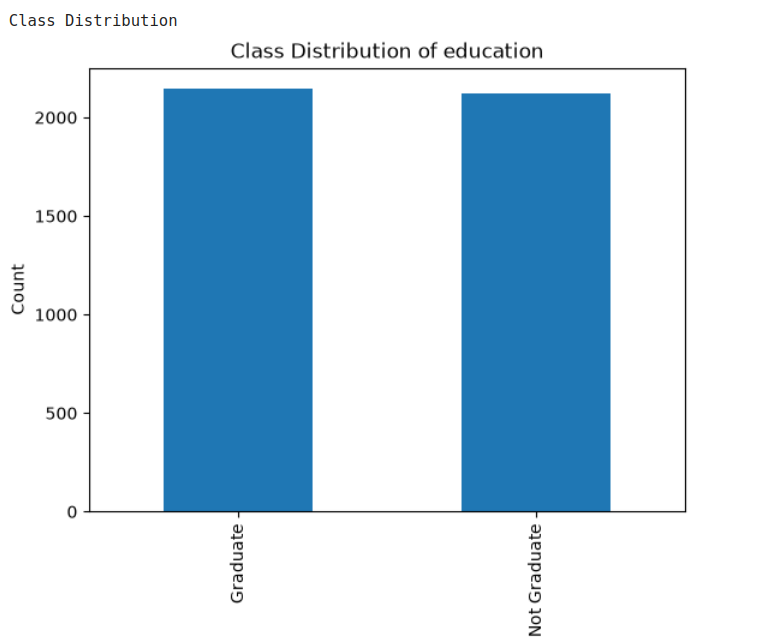
\includegraphics[width=0.7\linewidth]{images/loan_education_distribution.png}
\caption{Distribution of Education Level}
\end{figure}
\begin{figure}[H]
\centering
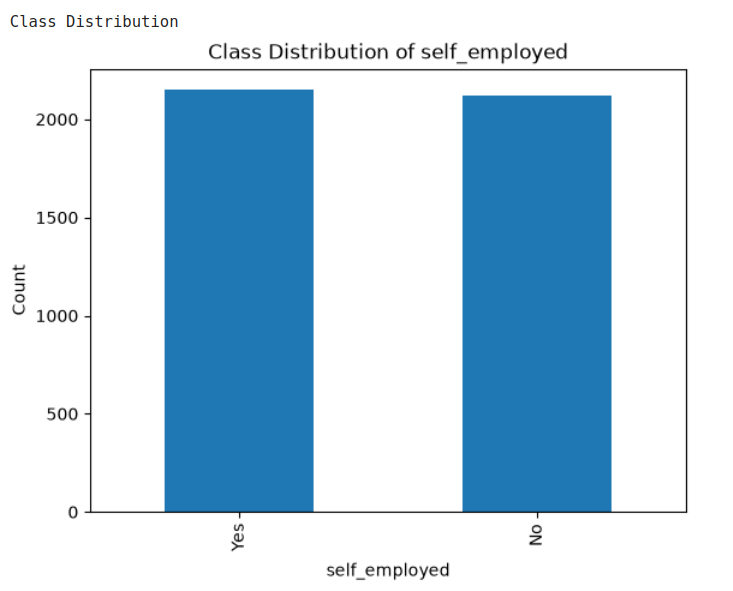
\includegraphics[width=0.7\linewidth]{images/loan_self_employed_distribution.png}
\caption{Distribution of Self Employment Status}
\end{figure}

\textbf{Inference:}
TODO: Discuss the balance in both categorical features.

\subsubsection{Histograms}
\begin{figure}[H]
\centering
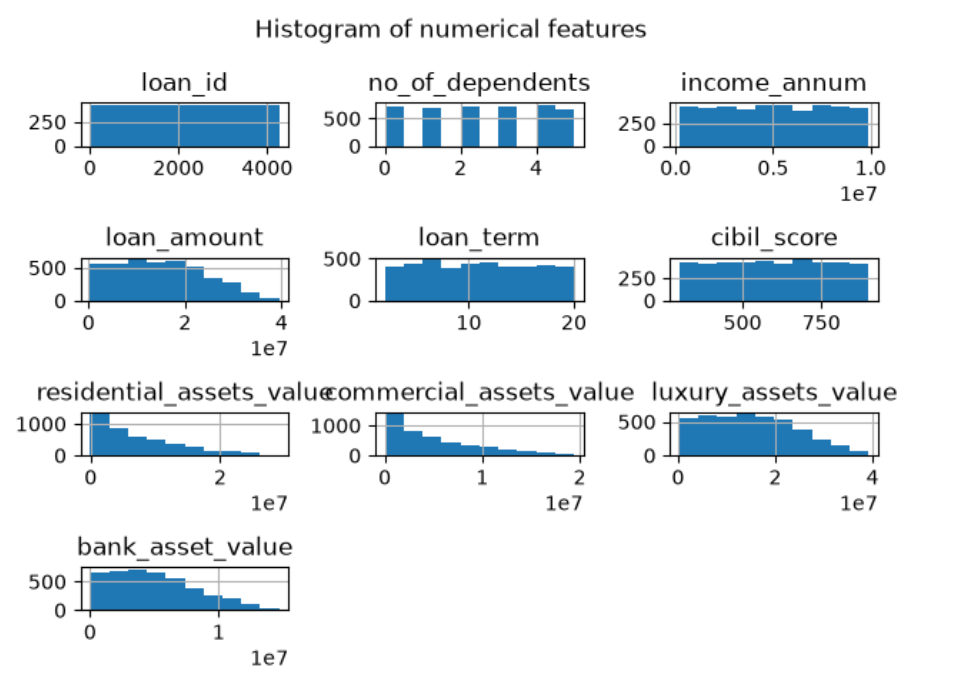
\includegraphics[width=0.7\linewidth]{images/loan_histograms.png.png}
\caption{Histograms of Numerical Features — Loan Dataset}
\end{figure}

\textbf{Inference:}
TODO: Describe the skewness observed in loan amount and asset value columns, and the uniform distribution of income, loan term, and CIBIL score.

\subsubsection{Box Plots}
The \texttt{plot\_boxplot()} function generates one separate box plot per numerical feature. The following box plots were saved for the Loan dataset:

\begin{figure}[H]
\centering
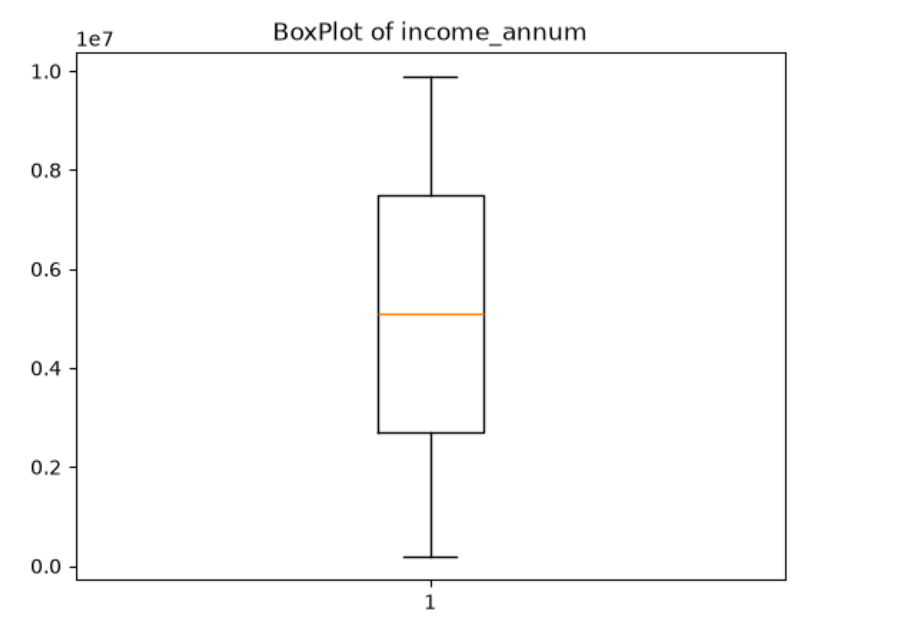
\includegraphics[width=0.6\linewidth]{images/loan_boxplot_income_annum.png}
\caption{Box Plot of Annual Income}
\end{figure}
\begin{figure}[H]
\centering
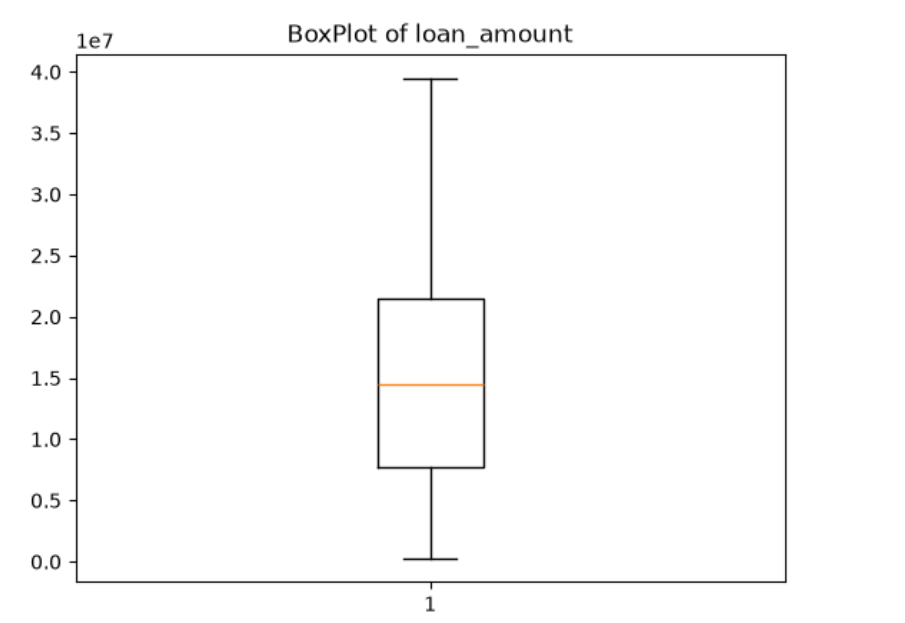
\includegraphics[width=0.6\linewidth]{images/loan_boxplot_loan_amount.png}
\caption{Box Plot of Loan Amount}
\end{figure}
\begin{figure}[H]
\centering
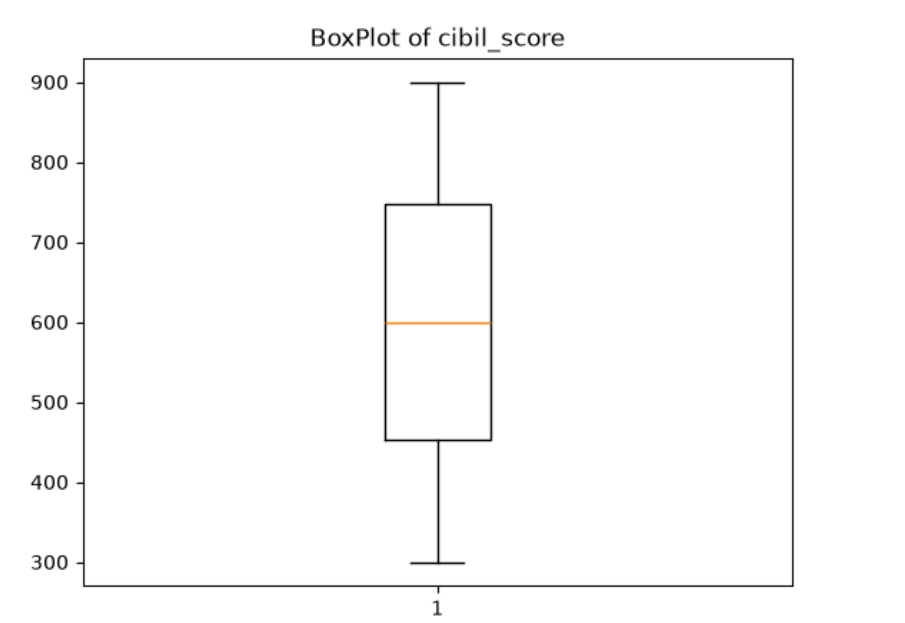
\includegraphics[width=0.6\linewidth]{images/loan_boxplot_cibil_score.png}
\caption{Box Plot of CIBIL Score}
\end{figure}

\textbf{Inference:}
TODO: Discuss outliers — income, loan amount, and CIBIL score show no outliers. Other numerical features (asset values) showed upper outliers.

\subsubsection{Correlation Heatmap}
\begin{figure}[H]
\centering
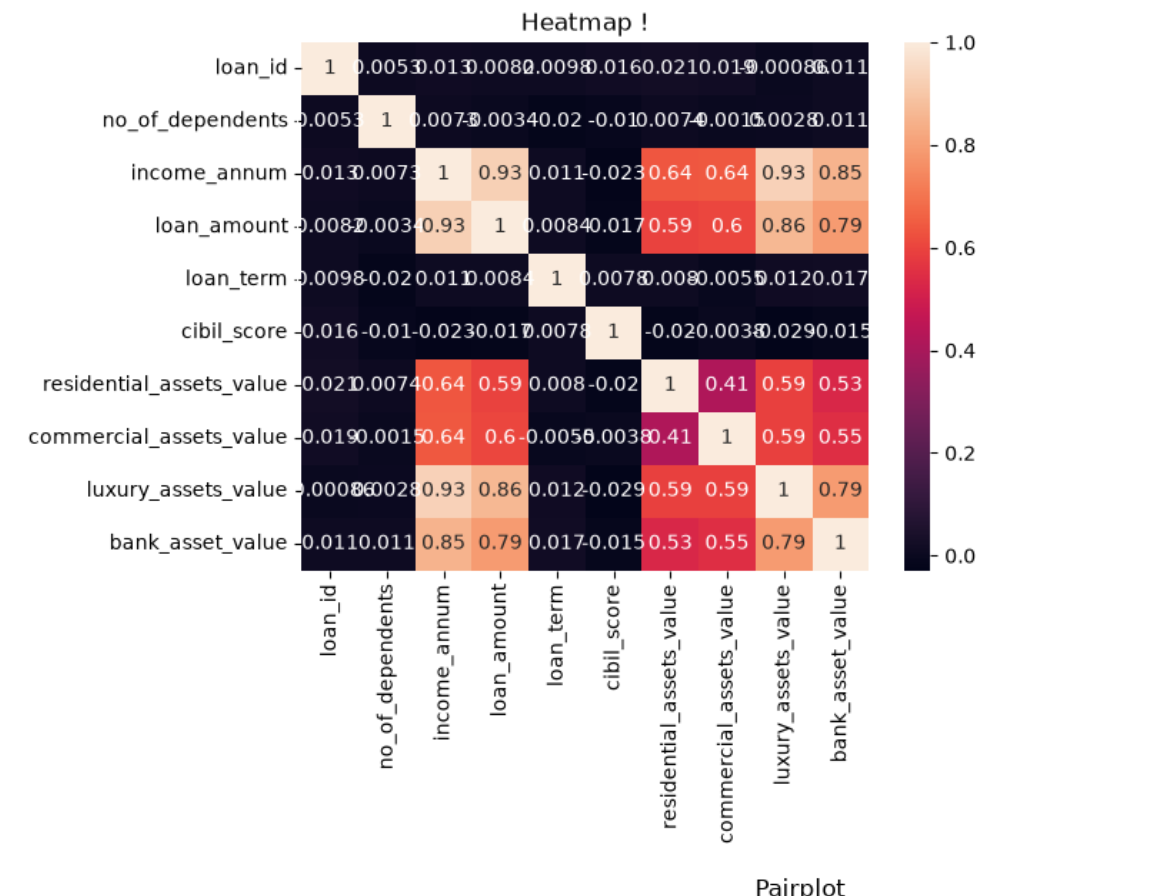
\includegraphics[width=0.7\linewidth]{images/loan_correlation_heatmap.png}
\caption{Correlation Heatmap — Loan Dataset}
\end{figure}

\textbf{Inference:}
TODO: Interpret the strong positive correlation between income\_annum and loan\_amount (0.93), and the very low correlation of CIBIL score with other features.

\subsubsection{Pair Plot (Selected Features)}
\begin{figure}[H]
\centering
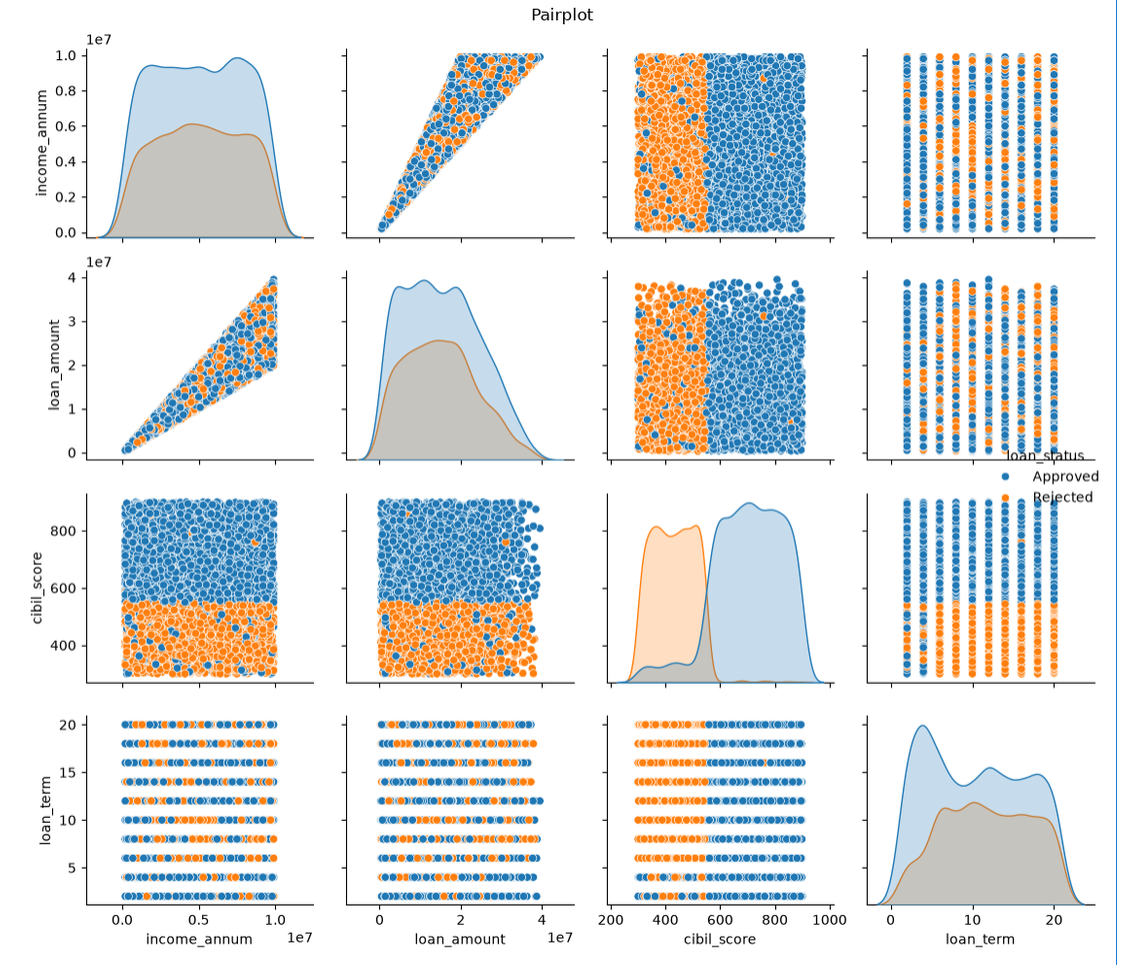
\includegraphics[width=0.7\linewidth]{images/loan_pairplot.png}
\caption{Pair Plot of Key Features colored by Loan Status}
\end{figure}

\textbf{Inference:}
TODO: Explain how CIBIL score shows the clearest separation between approved and rejected applications, while other features show heavy overlap.

\section{Dataset 3: Diabetes Prediction Dataset (Classification)}

\subsection{Dataset Description}
\begin{longtable}{|p{5cm}|p{9cm}|}
\hline
Dataset Name & Diabetes Prediction \\ \hline
Dataset Source & \texttt{Diabetes\_Prediction/diabetes\_prediction\_dataset.csv} \\ \hline
Number of Samples & 100,000 \\ \hline
Number of Features & 9 (including target) \\ \hline
Target Variable & \texttt{diabetes} (0 = Non-Diabetic, 1 = Diabetic) \\ \hline
Missing Values & None \\ \hline
Duplicate Records & 3,854 \\ \hline
\end{longtable}

TODO: Describe the dataset and the binary classification task.

\subsection{Loading and Basic Information}
TODO: Discuss dataset size, features, data types, and initial observations.

\subsection{Missing Values and Duplicates}
TODO: Report that no missing values exist but 3,854 duplicate records were detected — discuss potential impact on model training.

\subsection{Summary Statistics}
TODO: Present key statistics — age range, BMI, HbA1c levels, blood glucose levels.

\begin{longtable}{|l|r|r|r|r|}
\hline
\textbf{Feature} & \textbf{Mean} & \textbf{Std} & \textbf{Min} & \textbf{Max} \\ \hline
age & TODO & TODO & TODO & TODO \\ \hline
bmi & TODO & TODO & TODO & TODO \\ \hline
HbA1c\_level & TODO & TODO & TODO & TODO \\ \hline
blood\_glucose\_level & TODO & TODO & TODO & TODO \\ \hline
\end{longtable}

\subsection{Exploratory Data Analysis}

\subsubsection{Histograms}
\begin{figure}[H]
\centering
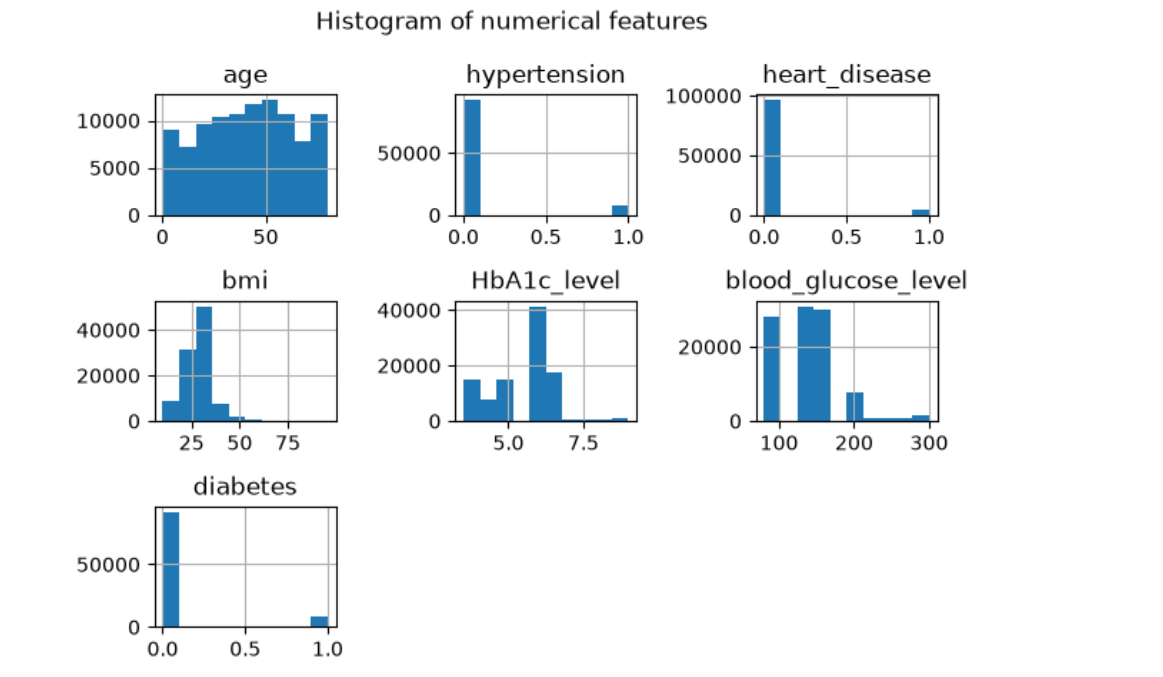
\includegraphics[width=0.7\linewidth]{images/diabetes_histograms.png}
\caption{Histograms of Numerical Features — Diabetes Dataset}
\end{figure}

\textbf{Inference:}
TODO: Discuss the distribution of age, BMI, HbA1c, blood glucose, and the imbalance in the target variable.

\subsubsection{Box Plots}
The \texttt{plot\_boxplot()} function generates one separate box plot per numerical feature. The following box plots were saved for the Diabetes dataset:

\begin{figure}[H]
\centering
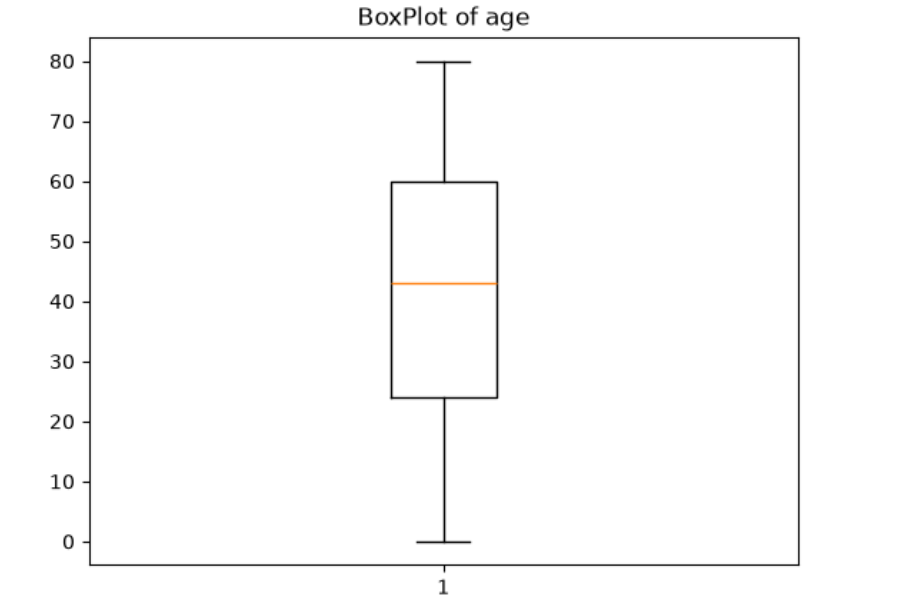
\includegraphics[width=0.6\linewidth]{images/diabetes_boxplot_age.png}
\caption{Box Plot of Age}
\end{figure}
\begin{figure}[H]
\centering
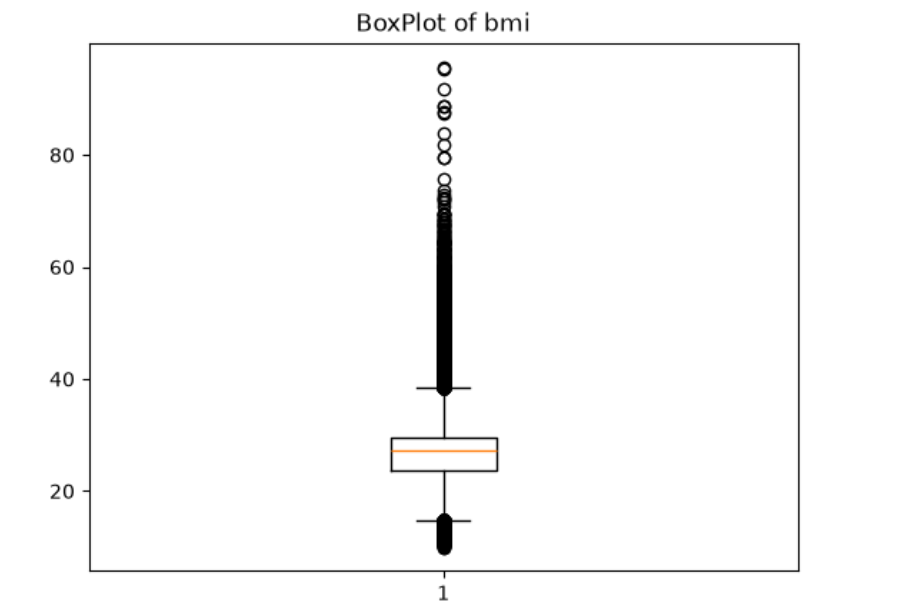
\includegraphics[width=0.6\linewidth]{images/diabetes_boxplot_bmi.png}
\caption{Box Plot of BMI}
\end{figure}
\begin{figure}[H]
\centering
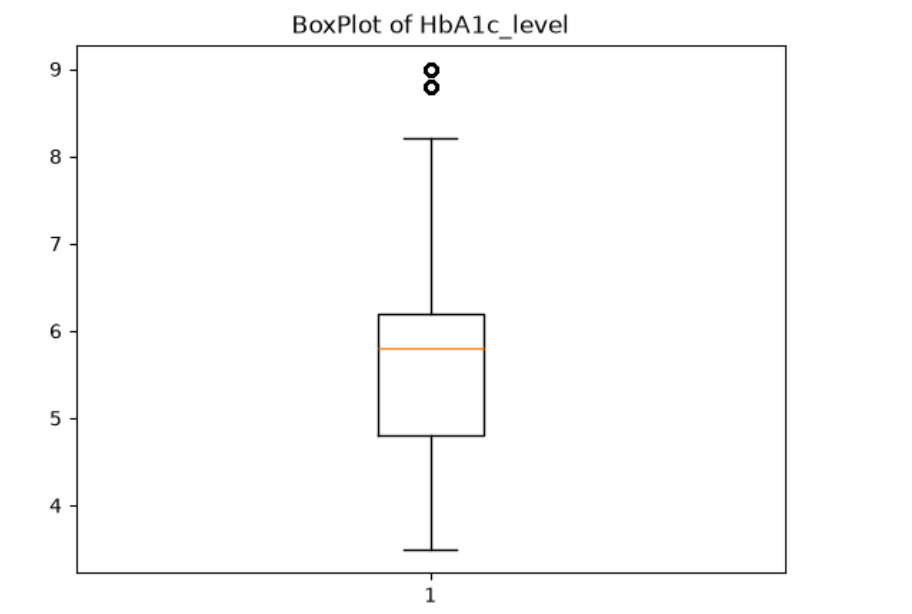
\includegraphics[width=0.6\linewidth]{images/diabetes_boxplot_hba1c.png}
\caption{Box Plot of HbA1c Level}
\end{figure}
\begin{figure}[H]
\centering
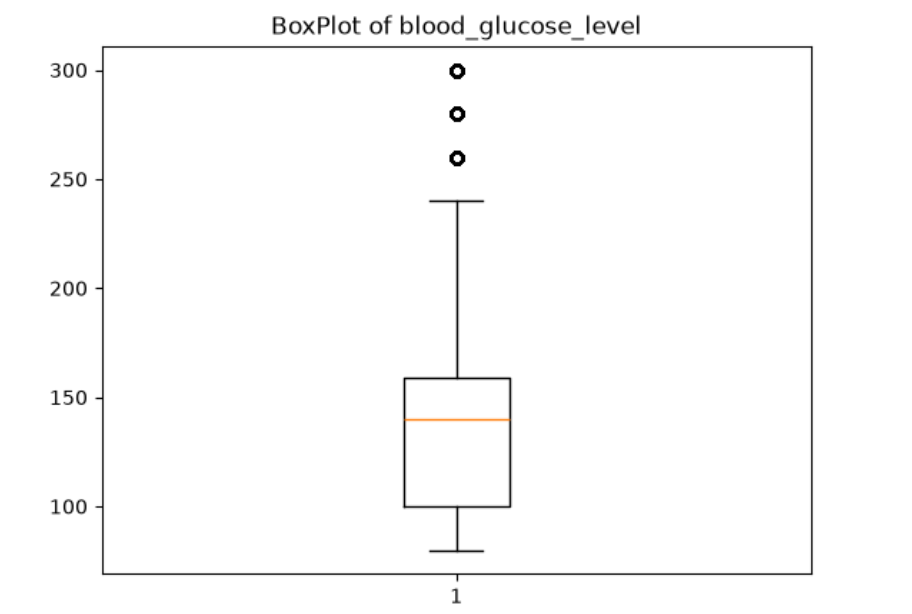
\includegraphics[width=0.6\linewidth]{images/diabetes_boxplot_blood_glucose.png}
\caption{Box Plot of Blood Glucose Level}
\end{figure}

\textbf{Inference:}
TODO: Discuss outliers — BMI contains numerous upper outliers; HbA1c level and blood glucose level also show high-value outliers.

\subsubsection{Correlation Heatmap}
\begin{figure}[H]
\centering
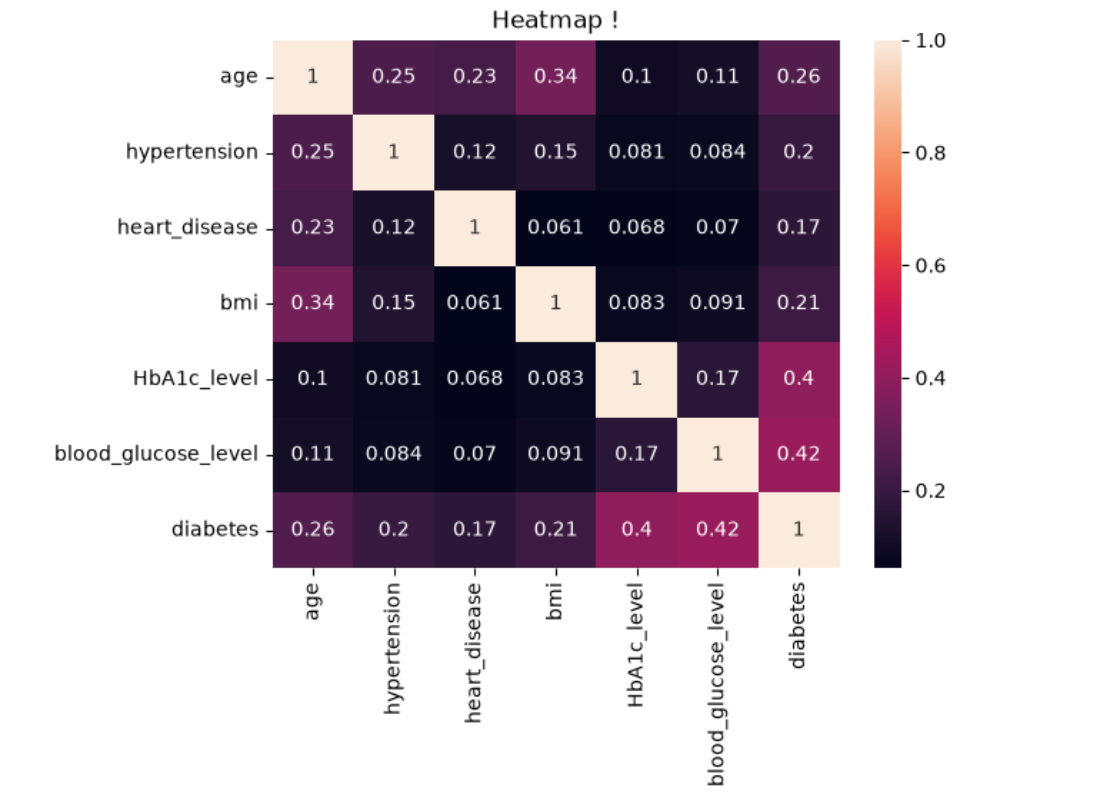
\includegraphics[width=0.7\linewidth]{images/diabetes_correlation_heatmap.png}
\caption{Correlation Heatmap — Diabetes Dataset}
\end{figure}

\textbf{Inference:}
TODO: Interpret correlations — blood glucose level (0.42) and HbA1c level (0.40) have the highest correlation with diabetes.

\section{Dataset 4: Handwritten Digits Dataset (Classification)}

\subsection{Dataset Description}
\begin{longtable}{|p{5cm}|p{9cm}|}
\hline
Dataset Name & Digits \\ \hline
Dataset Source & scikit-learn \texttt{load\_digits()} (built-in) \\ \hline
Number of Samples & 1,797 \\ \hline
Number of Features & 64 (8×8 pixel values) \\ \hline
Number of Classes & 10 (digits 0–9) \\ \hline
Missing Values & None \\ \hline
Duplicate Records & None \\ \hline
\end{longtable}

TODO: Describe the dataset and the multi-class classification task.

\subsection{Loading and Basic Information}
TODO: Explain how the dataset was loaded using \texttt{load\_digits()} and converted to a DataFrame with a target column.

\subsection{Exploratory Data Analysis}
For the Digits dataset, only class distribution was plotted (histograms, box plots, heatmap, and pair plot were intentionally skipped since the 64 pixel features are not individually meaningful for univariate analysis).

\subsubsection{Class Distribution}
\begin{figure}[H]
\centering
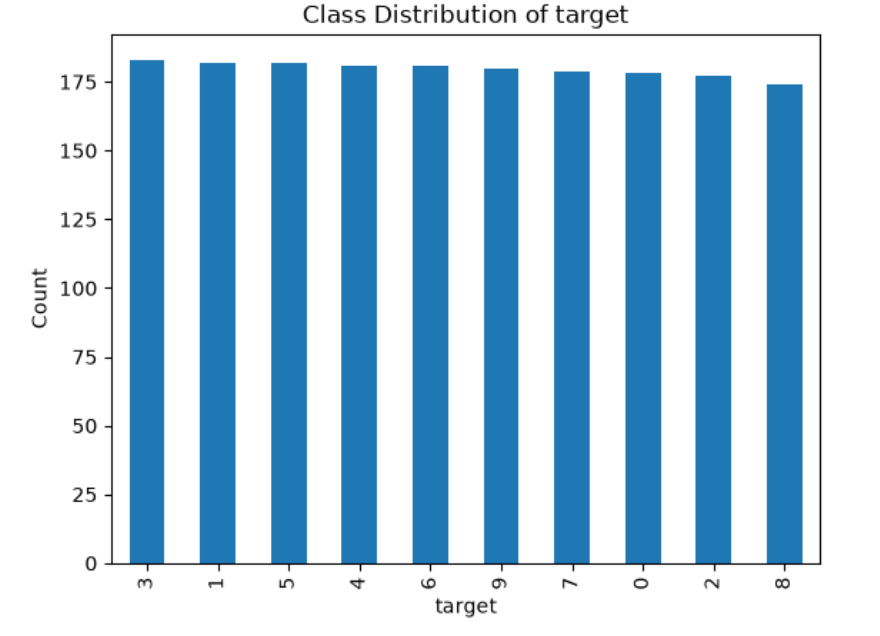
\includegraphics[width=0.7\linewidth]{images/digits_class_distribution.png}
\caption{Class Distribution of Digits 0–9}
\end{figure}

\textbf{Inference:}
TODO: Discuss whether the digit classes are balanced.

\subsubsection{Sample Visualization}
TODO: Insert sample digit images (8×8 pixel representations) here if available.

\textbf{Inference:}
TODO: Show sample images of each digit and describe the visual representation.

\section{Dataset 5: Email Spam Classification Dataset}

\subsection{Dataset Description}
\begin{longtable}{|p{5cm}|p{9cm}|}
\hline
Dataset Name & Email Spam \\ \hline
Dataset Source & \texttt{emailSpam/emails.csv} \\ \hline
Number of Samples & 5,172 \\ \hline
Number of Features & 3,002 (3,000 word frequency columns + Email No. + Prediction) \\ \hline
Target Variable & \texttt{Prediction} (0 = Not Spam, 1 = Spam) \\ \hline
Missing Values & None \\ \hline
Duplicate Records & None \\ \hline
\end{longtable}

TODO: Describe the dataset and the binary classification task.

\subsection{Loading and Basic Information}
TODO: Explain how the dataset was loaded and the initial observations about its high-dimensional nature (3000+ features).

\subsection{Exploratory Data Analysis}
For the Email Spam dataset, only class distribution was plotted (histograms, box plots, heatmap, and pair plot were intentionally skipped due to the extremely high dimensionality of the data).

\subsubsection{Class Distribution}
\begin{figure}[H]
\centering
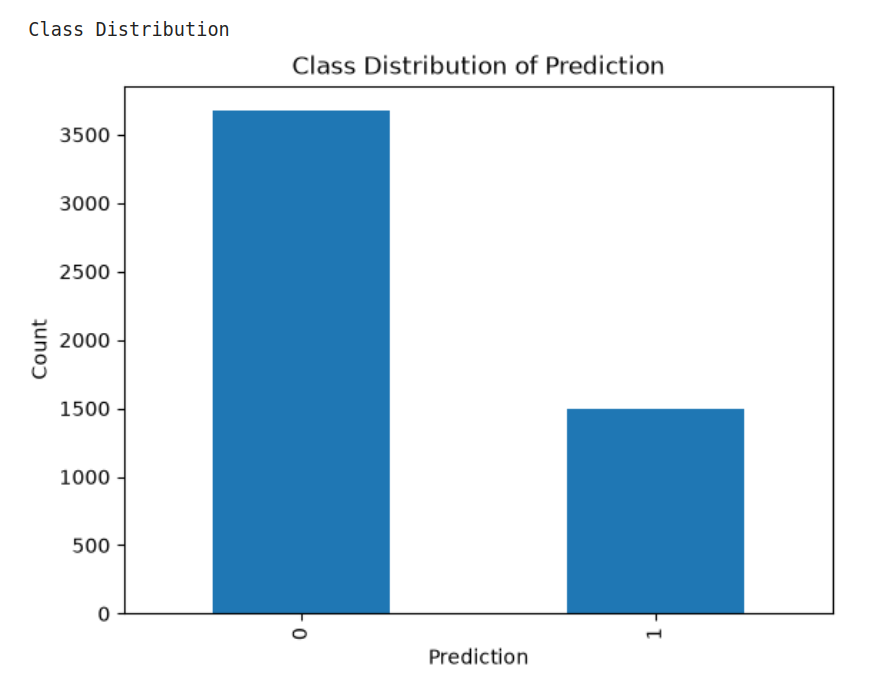
\includegraphics[width=0.7\linewidth]{images/spam_class_distribution.png}
\caption{Distribution of Spam vs Non-Spam Emails}
\end{figure}

\textbf{Inference:}
TODO: Discuss the balance (or imbalance) between spam and non-spam classes.

\section{Comparison Summary Across Datasets}

\begin{longtable}{|p{3.5cm}|c|c|c|c|c|}
\hline
\textbf{Property} & \textbf{Iris} & \textbf{Loan} & \textbf{Diabetes} & \textbf{Digits} & \textbf{Spam} \\ \hline
Samples & 150 & 4,269 & 100,000 & 1,797 & 5,172 \\ \hline
Features & 4 & 13 & 9 & 64 & 3,002 \\ \hline
Classes & 3 & 2 & 2 & 10 & 2 \\ \hline
Missing Values & 0 & 0 & 0 & 0 & 0 \\ \hline
Duplicates & 3 & 0 & 3,854 & 0 & 0 \\ \hline
Task Type & Multi-class Classification & Binary Classification & Binary Classification & Multi-class Classification & Binary Classification \\ \hline
\end{longtable}

TODO: Write a brief comparative analysis of the datasets in terms of size, complexity, and EDA findings.

\section{Key Observations and Discussion}
TODO: Write a consolidated discussion covering:

\begin{itemize}
    \item The importance of EDA in understanding datasets before model building.
    \item How visualizations (histograms, box plots, heatmaps, pair plots) reveal patterns, outliers, and feature relationships.
    \item The utility of reusable EDA functions for scaling analysis across multiple datasets.
    \item Notable findings such as the bimodal nature of Iris petal features, the strong correlation between income and loan amount, and the predictive power of CIBIL scores and HbA1c levels.
    \item The presence of duplicates in the Diabetes dataset and the need for preprocessing.
\end{itemize}

\section{Conclusion}
TODO: Summarize the experiment — the ability to load, explore, and visualize multiple datasets using a systematic EDA pipeline was demonstrated, providing critical insights that guide subsequent preprocessing and modeling decisions.

\section{Learning Outcomes}
TODO: Write 3–5 learning outcomes, such as:

\begin{itemize}
    \item Implemented reusable data loading and EDA functions in Python.
    \item Gained proficiency in using pandas, Matplotlib, and Seaborn for data analysis.
    \item Learned to interpret statistical summaries and visualizations to extract meaningful insights.
    \item Understood the importance of detecting missing values, duplicates, and outliers.
    \item Recognized how feature correlations and distributions inform feature selection and model choice.
\end{itemize}

\section{References}
\begin{enumerate}
    \item TODO: Reference the Iris dataset (UCI Repository).
    \item TODO: Reference scikit-learn documentation for load\_digits.
    \item TODO: Reference pandas documentation.
    \item TODO: Reference Matplotlib and Seaborn documentation.
\end{enumerate}

\end{document}